\documentclass{article}
\usepackage[utf8]{inputenc}
% are all of these packages really necessary?
% no.
% i'm just too lazy to only grab the packages i want for a specific
% document, so i just glob all of my most commonly used packages together
% this is bad practice.
\usepackage{amsmath,amsthm,amssymb,amsfonts, fancyhdr, color, comment, graphicx, environ, mdframed, soul, calc, enumitem, mdframed, xcolor, geometry, empheq, mathtools, tikz, pgfplots, caption, subcaption, hyperref}

\usetikzlibrary{external}
\tikzexternalize[prefix=tikz/,optimize command away=\includepdf]

%tikzpicture
\usepackage{tikz}
\usepackage{scalerel}
\usepackage{pict2e}
\usepackage{tkz-euclide}
\usetikzlibrary{calc}
\usetikzlibrary{patterns,arrows.meta}
\usetikzlibrary{shadows}
\usetikzlibrary{external}

%pgfplots
\usepackage{pgfplots}
\pgfplotsset{compat=newest}
\usepgfplotslibrary{statistics}
\usepgfplotslibrary{fillbetween}
\usepgfplotslibrary{polar}

\tikzset{external/export=true}
\pgfplotsset{
    standard/.style={
    axis line style = thick,
    trig format=rad,
    enlargelimits,
    axis x line=middle,
    axis y line=middle,
    enlarge x limits=0.15,
    enlarge y limits=0.15,
    every axis x label/.style={at={(current axis.right of origin)},anchor=north west},
    every axis y label/.style={at={(current axis.above origin)},anchor=south east}
    }
}
\newcommand*\widefbox[1]{\fbox{\hspace{2em}#1\hspace{2em}}}
% Command "alignedbox{}{}" for a box within an align environment
% Source: http://www.latex-community.org/forum/viewtopic.php?f=46&t=8144
\newlength\dlf  % Define a new measure, dlf
\newcommand\alignedbox[2]{
% Argument #1 = before & if there were no box (lhs)
% Argument #2 = after & if there were no box (rhs)
&  % Alignment sign of the line
{
\settowidth\dlf{$\displaystyle #1$}  
    % The width of \dlf is the width of the lhs, with a displaystyle font
\addtolength\dlf{\fboxsep+\fboxrule}  
    % Add to it the distance to the box, and the width of the line of the box
\hspace{-\dlf}  
    % Move everything dlf units to the left, so that & #1 #2 is aligned under #1 & #2
\boxed{#1 #2}
    % Put a box around lhs and rhs
}
}

\hypersetup{
    colorlinks=true,
    linkcolor=blue,
    filecolor=magenta,      
    urlcolor=cyan,
    pdftitle={Homework 10 Solutions},
    pdfpagemode=UseOutlines,
    bookmarksopen=true,
    pdfauthor={Christina Phan}
}
\newcommand{\lrp}[1]{\left( #1 \right)}
\newcommand{\abs}[1]{\left\vert #1 \right\vert}
\newcommand{\lra}[1]{\left\langle #1 \right\rangle}
\newcommand{\lrb}[1]{\left[ #1 \right]}
\newcommand{\norm}[1]{\left\lVert #1 \right\rVert}
\newcommand{\iintR}[0]{\iint\limits_{R}}
\renewcommand{\u}[0]{\mathbf{u}}
\renewcommand{\i}[0]{\mathbf{i}}
\renewcommand{\j}[0]{\mathbf{j}}
\renewcommand{\k}[0]{\mathbf{k}}
\newcommand{\T}[0]{\mathbf{T}}
\newcommand{\N}[0]{\mathbf{N}}
\newcommand{\B}[0]{\mathbf{B}}
\renewcommand{\r}[0]{\mathbf{r}}
\renewcommand{\a}[0]{\mathbf{a}}
\renewcommand{\v}[0]{\mathbf{v}}

\geometry{letterpaper, portrait, margin=1in}
\renewcommand{\footrulewidth}{0.8pt}
\setlength\parindent{0pt}
\pagestyle{fancy}
\lhead{Christina Phan}
\rhead{MAT 21D} 
\chead{\textbf{Homework 10 Solutions}}

\newcommand{\Solution}{\textit{Solution}}
\pgfplotsset{compat=1.18}
\begin{document}
\phantomsection
\addcontentsline{toc}{section}{Problem 1}\textbf{Problem 1}

Find the osculating circle to the curve $x=2\cos y- 2$ at the point $(0,0)$.

\Solution

You can go through all those steps with the $\r=\lra{2\cos t, t}$, $\r'(t)$, $\T$, etc, but I don't want to :)

I will use the formula from Homework 9 which states
\begin{align*}
    \kappa (y)&=\frac{\left|f''(y)\right|}{(1+f'(y)^2)^{3/2}}
\end{align*}
Let's find $f'(y)$, $f''(y)$, and $\kappa(0)$.
\begin{align*}
    f'(y)&=-2\sin y\\
    f''(y)&=-2\cos y\\
    \kappa(y) &=\frac{\left|-2\cos y\right|}{\big(1+(-2\sin y)^2\big)^{3/2}}\\
    \kappa(0)&=\frac{\left|-2\cos0\right|}{(1-(2\sin^2 0)^2)^{3/2}}=\frac{2}{(1-0)^{3/2}}=2
\end{align*}

The radius of the osculating circle is
\begin{align*}
    r&=\frac{1}{\kappa}
\end{align*}
For $\kappa(0)=2$,
\begin{align*}
    r=\frac{1}{2}
\end{align*}
Let's graph $x=2\cos y-2$ to get an idea of where the center our our osculating circle might be. Remember: the osculating circle must be \textit{inside} the concavity of the function.
\begin{center}
\resizebox{3.5cm}{!}{
    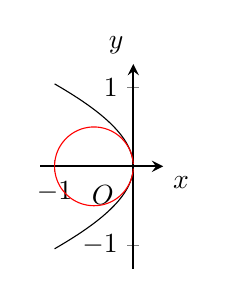
\begin{tikzpicture}
    \begin{axis}[standard,
            xtick={-1},
            ytick={-1,1},
            samples=1000,
            xlabel={$x$},
            ylabel={$y$},
            xmin=-1,xmax=0.2,
            ymin=-1,ymax=1,
            x=1cm,
            y=1cm/1
           ]
\node[anchor=center,label=south west:$O$] at (axis cs:0,0){};
\addplot[name path=F,domain={-1:0}]{acos(0.5*x+1)};
\addplot[name path=G,domain={-1:0}]{-acos(0.5*x+1)};
\addplot[name path = H, domain={-1:0},color=red]{sqrt(0.25-(x+0.5)^2)};
\addplot[name path = H, domain={-1:0},color=red]{-sqrt(0.25-(x+0.5)^2)};
    \end{axis}
    \end{tikzpicture}
}
\end{center}
By symmetry (and visually), the $y$ value of our center must be $0$.

We know that our radius is $\dfrac{1}{2}$, so the $x$ value of our center must be $0-\dfrac{1}{2}=-\dfrac{1}{2}$. 

Putting this all together, we get osculating circle equation which is
\begin{align*}
    \alignedbox{\lrp{x+\frac{1}{2}}^2+y^2}{=\frac{1}{4}}
\end{align*}
\newpage
\phantomsection
\addcontentsline{toc}{section}{Problem 2}\textbf{Problem 2} 

Show that the center of the osculating circle for the parabola $y=x^2$ at the point $(a,a^2)$ is located at $\displaystyle\lrp{-4a^3,3a^2+\frac{1}{2}}$.

\Solution

You can go through all those steps with the $\r=\lra{t, t^2}$, $\r'(t)$, $\T$, etc, but I don't want to :)

I will use the formula from Homework 9 which states
\begin{align*}
    \kappa (x)&=\frac{\left|f''(x)\right|}{(1+f'(x)^2)^{3/2}}
\end{align*}
Let's find $f'(x)$, $f''(x)$, and $\kappa(a)$.
\begin{align*}
    f'(x)&=2x\\
    f''(x)&=2\\
    \kappa(x)&=\frac{\left|2\right|}{\big(1+(2x)^2\big)^{3/2}}=\frac{2}{(1+4x^2)^{3/2}}\\
    \kappa(a)&=\frac{2}{(1+4a^2)^{3/2}}
\end{align*}
The radius of the osculating circle is
\begin{align*}
    r&=\frac{1}{\kappa}
\end{align*}
For $\displaystyle \kappa(a)=\frac{2}{(1+4a^2)^{3/2}}$,
\begin{align*}
    r&=\frac{1}{\frac{2}{(1+4a^2)^{3/2}}}=\frac{1}{2}(1+4a^2)^{3/2}
\end{align*}
If the center of the osculating circle for the parabola $y=x^2$ at the point $(a,a^2)$ is located at $\displaystyle\lrp{-4a^3,3a^2+\frac{1}{2}}$, then the distance between $(a,a^2)$ and $\displaystyle\lrp{-4a^3,3a^2+\frac{1}{2}}$ must be equal to the radius $r=\dfrac{1}{2}(1+4a^2)^{3/2}$.

Let's find the distance between $(a,a^2)$ and $\displaystyle\lrp{-4a^3,3a^2+\frac{1}{2}}$.
\begin{align*}
    d&=\sqrt{\big(a-(-4a^3)\big)^2 + \bigg(a^2 -\lrp{3a^2+\frac{1}{2}}\bigg)^2}\\
    &=\sqrt{(a+4a^3)^2+\lrp{-2a^2-\frac{1}{2}}^2}\\
    &=\sqrt{(a^2 + 8a^4 + 16a^6)+\lrp{4a^4 +2a^2 + \frac{1}{4}}}\\
    &=\sqrt{16a^6 + 12a^4 + 3a^2 + \frac{1}{4}}\\
    &=\sqrt{\frac{1}{4}\lrp{64a^6+48a^4+12a^2+1}}\\
    &=\frac{1}{2}\sqrt{(4a^2+1)^3}\tag{trust me i swear... or, use binomial theorem}\\
    &=\frac{1}{2}(1+4a^2)^{3/2}
\end{align*}

Since the distance between $(a,a^2)$ and $\displaystyle\lrp{-4a^3,3a^2+\frac{1}{2}}$ is $\displaystyle \frac{1}{2}(1+4a^2)^{3/2}$ and the radius of the osculating circle for the parabola $y=x^2$ at the point $(a,a^2)$ is also $\displaystyle \frac{1}{2}(1+4a^2)^{3/2}$, the distance between $(a,a^2)$ and $\displaystyle\lrp{-4a^3,3a^2+\frac{1}{2}}$ is equal to the radius of the osculating circle.

Also, if the center of the osculating circle for the parabola $y=x^2$ at the point $(a,a^2)$ is located at $\displaystyle\lrp{-4a^3,3a^2+\frac{1}{2}}$, then the tangent line at $(a,a^2)$ ($\T$) must be perpendicular to the line between $(a,a^2)$ and $\displaystyle\lrp{-4a^3,3a^2+\frac{1}{2}}$ ($\N$). This is pretty much the ``center of osculating circle is in direction of $\N$" idea from lecture, except I don't want to write the vectors for those so we're just going to think ``abstractly".
\begin{align*}
    y'&=2x\\
    y'(a)&=2a\\
    \implies \text{tangent slope}&=2a\\
    \text{slope between}&=\frac{\lrp{3a^2+\frac{1}{2}}-a^2}{-4a^3-a}=\frac{2a^2+\frac{1}{2}}{-4a^3-a}=\frac{2a^2+\frac{1}{2}}{-2a\lrp{2a^2+\frac{1}{2}}}=-\frac{1}{2a}
\end{align*}
Since negative one over the tangent slope is equal to the slope in between the two points, the tangent line and line in between are perpendicular to each other by definition of perpendicular slopes.

Since both conditions for the center of an osculating circle are satisfied, $\displaystyle\lrp{-4a^3,3a^2+\frac{1}{2}}$ must be the center of the osculating circle for the parabola $y=x^2$.

\qed
\newpage
\phantomsection
\addcontentsline{toc}{section}{Problem 3 (Parts)}\textbf{Problem 3 (Parts)} 

In Homework 9, you found the vectors $\T$ and $\N$ for these curves. Find the vector $\B$:

\phantomsection
\addcontentsline{toc}{subsection}{3(a)}\textbf{(a)} $\r(t)=\lra{e^t\cos t,e^t\sin t,2}$

\Solution

This is problem 1(c) on Homework 9.

For $\T$ and $\N$, please refer back to your own Homework 9 solutions, or my Homework 9 solutions (campuswire \#45).

Recall that $\B$ equal to the cross product of $\T$ and $\N$. That is,
\begin{align*}
    \B&=\T \times \N
\end{align*}
Let's find $\B$ in this problem.

If you have taken or are taking linear algebra, you would know that there is a slightly faster way to find the determinate. I am doing it this way (21C way) as linear algebra is not a prereq for 21D.
\begin{align*}
    \T&=\lra{\frac{\cos t-\sin t}{\sqrt{2}},\frac{\sin t + \cos t}{\sqrt{2}},0}\\
    \N&=\lra{\frac{-\sin t-\cos t}{\sqrt{2}},\frac{\cos t-\sin t}{\sqrt{2}},0}\\
    \B&=\lra{\frac{\cos t-\sin t}{\sqrt{2}},\frac{\sin t + \cos t}{\sqrt{2}},0}\times \lra{\frac{-\sin t-\cos t}{\sqrt{2}},\frac{\cos t-\sin t}{\sqrt{2}},0}\\
    &=\begin{vmatrix}
\mathbf{i} & \mathbf{j} & \mathbf{k}\\
\frac{\cos t-\sin t}{\sqrt{2}} & \frac{\sin t + \cos t}{\sqrt{2}} & 0\\
\frac{-\sin t-\cos t}{\sqrt{2}} & \frac{\cos t-\sin t}{\sqrt{2}} & 0\\
\end{vmatrix}\\
&=\begin{vmatrix}
\frac{\sin t + \cos t}{\sqrt{2}} & 0\\
\frac{\cos t-\sin t}{\sqrt{2}} &0\\
\end{vmatrix}\mathbf{i}-
\begin{vmatrix}
\frac{\cos t-\sin t}{\sqrt{2}} & 0\\
\frac{-\sin t-\cos t}{\sqrt{2}} & 0\\
\end{vmatrix}\mathbf{j}+
\begin{vmatrix}
\frac{\cos t-\sin t}{\sqrt{2}} & \frac{\sin t + \cos t}{\sqrt{2}}\\
\frac{-\sin t-\cos t}{\sqrt{2}} & \frac{\cos t-\sin t}{\sqrt{2}}\\
\end{vmatrix}\mathbf{k}\\
&=(0-0)\mathbf{i}-(0-0)\mathbf{j}+\Bigg(\left(\frac{\cos t-\sin t}{\sqrt{2}}\right)\left(\frac{\cos t-\sin t}{\sqrt{2}}\right)-\left(\frac{\sin t + \cos t}{\sqrt{2}}\right)\left(\frac{-\sin t-\cos t}{\sqrt{2}}\right)\Bigg)\mathbf{k}\\
&=\Bigg(\frac{\cos^2 t - 2\sin t\cos t+\sin ^2 t}{2}-\frac{-\sin^2 t -2\sin t\cos t -\cos^2}{2}\Bigg)\k\\
&=\Bigg(\frac{-2\sin t\cos t+ 1}{2}-\frac{-2\sin t\cos t-1}{2}\Bigg)\k\tag{$\sin ^2 t+\cos ^2 t = 1$}\\
&=\lrp{\frac{0+2}{2}}\k\\
&=\k\\
&=\boxed{\lra{0,0,1}}
\end{align*}
\newpage
\phantomsection
\addcontentsline{toc}{subsection}{3(b)}\textbf{(b)} $\r(t)=\lra{6\sin 2t,6\cos 2t, 5t}$

This is problem 1(d) on Homework 9.

For $\T$ and $\N$, please refer back to your own Homework 9 solutions, or my Homework 9 solutions (campuswire \#45).

Recall that $\B$ equal to the cross product of $\T$ and $\N$. That is,
\begin{align*}
    \B&=\T \times \N
\end{align*}
Let's find $\B$ in this problem.

If you have taken or are taking linear algebra, you would know that there is a slightly faster way to find the determinate. I am doing it this way (21C way) as linear algebra is not a prereq for 21D.
\begin{align*}
    \T&=\lra{\frac{12\cos 2t}{13},\frac{-12\sin 2t}{13},\frac{5}{13}}\\
    \N&=\lra{-\sin 2t, -\cos 2t, 0}\\
    \B&=\lra{\frac{12\cos 2t}{13},\frac{-12\sin 2t}{13},\frac{5}{13}}\times \lra{-\sin 2t, -\cos 2t, 0}\\
    &=\begin{vmatrix}
\mathbf{i} & \mathbf{j} & \mathbf{k}\\
\frac{12\cos 2t}{13} & \frac{-12\sin 2t}{13} & \frac{5}{13}\\
-\sin 2t & -\cos 2t & 0\\
\end{vmatrix}\\
&=\begin{vmatrix}
\frac{-12\sin 2t}{13} & \frac{5}{13}\\
-\cos 2t & 0\\
\end{vmatrix}\mathbf{i}-
\begin{vmatrix}
\frac{12\cos 2t}{13} & \frac{5}{13}\\
-\sin 2t & 0\\
\end{vmatrix}\mathbf{j}+
\begin{vmatrix}
\frac{12\cos 2t}{13} & \frac{-12\sin 2t}{13}\\
-\sin 2t & -\cos 2t\\
\end{vmatrix}\mathbf{k}\\
&=\Bigg(0-\frac{5}{13}\lrp{-\cos 2t}\Bigg)\i-\Bigg(0-\frac{5}{13}\lrp{-\sin 2t}\Bigg)\j+\Bigg(\left(\frac{12\cos 2t}{13}\right)\left(-\cos 2t\right)-\left(\frac{-12\sin 2t}{13}\right)\left(-\sin 2t\right)\Bigg)\mathbf{k}\\
&=\lrp{\frac{5}{13}\cos 2t}\i-\lrp{\frac{5}{13}\sin 2t}\j+\Bigg(\frac{-12\cos^2 2t-12\sin^2 2t}{13}\Bigg)\k\\
&=\lrp{\frac{5}{13}\cos 2t}\i-\lrp{\frac{5}{13}\sin 2t}\j+\Bigg(\frac{-12(\cos^2 2t+\sin^2 2t)}{13}\Bigg)\k\\
&=\lrp{\frac{5}{13}\cos 2t}\i-\lrp{\frac{5}{13}\sin 2t}\j+\lrp{\frac{-12}{13}}\k\tag{$\sin^2 2t+\cos^2 2t=1$}\\
&=\boxed{\lra{\frac{5}{13}\cos 2t,-\frac{5}{13}\sin 2t,-\frac{12}{13}}}
\end{align*}
\phantomsection
\addcontentsline{toc}{section}{Problem 4 (Parts)}\textbf{Problem 4 (Parts)} 

Recall that we wrote the acceleration vector $\mathbf{a}(t)=\r''(t)$ as $\mathbf{a}=a_{\T}\T+a_{\N}\N$, where $a_{\T}\T=\dfrac{d}{dt}\lVert\mathbf{v}\rVert$ and $a_{\N}=\kappa\lVert\mathbf{v}\rVert^2$ are the \textit{tangential} and \textit{normal} components of acceleration. Since $\lVert \mathbf{a}\rVert^2=\mathbf{a}\cdot\mathbf{a}=a_{\T}^2+a_{\N}^2$, we can calculate $a_{\N}=\sqrt{\lVert\mathbf{a}\rVert^2 -a_{\T}^2}$ without needing to find $\kappa$. Use this to write $\mathbf{ a}=a_{\T}\T+a_{\N}\N$ for the curve at the value of $\T$:

\phantomsection
\addcontentsline{toc}{subsection}{4(a)}\textbf{(a)} $\r(t)=\lra{t+1,2t,t^2},t=1$

\Solution

Let's find $\v$, $\norm{\v}$, $\dfrac{d}{dt}\norm{\v}$, $\a$, and $\norm{\a}$.
\begin{align*}
    \v&=\lra{1,2,2t}\\
    \norm{\v}&=\sqrt{(1)^2+(2)^2+(2t)^2}=\sqrt{5+4t^2}\\
    \dfrac{d}{dt}\norm{\v}&=\frac{1}{2}(5+4t^2)^{-1/2}(8t)=4t(5+4t^2)^{-1/2}\\
    \a &= \lra{0,0,2}\\
    \norm{\a}&=\sqrt{(0)^2+(0)^2+(2)^2}=2
\end{align*}
At $t=1$,
\begin{align*}
    a_{\T}(1)&=\left.\frac{d}{dt}\right|_{t=1}\norm{\v}=4(1)\big(5+4(1)^2\big)^{-1/2}=\frac{4}{9^{1/2}}=\frac{4}{3}\\
    a_{\N}(1)&=\sqrt{\lrp{\norm{\a(1)}}^2-\lrp{a_{\T}(1)}^2}=\sqrt{\lrp{2}^2-\lrp{\frac{4}{3}}^2}=\sqrt{4-\frac{16}{9}}=\sqrt{\frac{20}{9}}=\frac{2\sqrt{5}}{3}
\end{align*}
Our final answer is
\begin{align*}
    \alignedbox{\a(1)}{=\frac{4}{3}\T+\frac{2\sqrt{5}}{3}\N}
\end{align*}
\phantomsection
\addcontentsline{toc}{subsection}{4(b)}\textbf{(b)} $\r(t)=\lra{e^t\cos t, e^t\sin t,\sqrt{2}e^t},t=0$

\Solution

Let's find $\v$, $\norm{\v}$, $\dfrac{d}{dt}\norm{\v}$, $\a$, and $\norm{\a}$.
\begin{align*}
    \v&=\lra{e^t\cos t-e^t\sin t, e^t\sin t+e^t\cos t, \sqrt{2}e^t}\\
    \norm{\v}&=\sqrt{(e^t\cos t-e^t\sin t)^2+(e^t\sin t+e^t\cos t)^2+(\sqrt{2}e^t)^2}\\
    &=\sqrt{\lrp{e^{2t}\cos^2 t -2e^{2t}\sin t\cos t+e^{2t}\sin^2 t}+\lrp{e^{2t}\sin^2 t + 2e^{2t}\sin t \cos t+e^{2t}\cos^2 t}+2e^{2t}}\\
    &=\sqrt{2e^{2t}\cos^2t +2e^{2t}\sin ^2 t + 2e^{2t}}\\
    &=\sqrt{2e^{2t}(\cos ^2 2t+\sin ^2 2t)+2e^{2t}}\\
    &=\sqrt{2e^{2t}+2e^{2t}}\tag{$\cos ^2 2t + \sin ^2 2t= 1$}\\
    &=\sqrt{4e^{2t}}\\
    &=2e^t\\
    \dfrac{d}{dt}\norm{\v}&=2e^t\\
    \a &= \lra{e^t\cos t - e^t\sin t - e^t\sin t - e^t\cos t, e^t\sin t + e^t\cos t + e^t\cos t - e^t\sin t,\sqrt{2}e^t}\\
    &=\lra{-2e^t\sin t,2e^t\cos t,\sqrt{2}e^t}\\
    \norm{\a}&=\sqrt{(2e^t\sin t)^2+(2e^t\cos t)^2+(\sqrt{2}e^t)^2}\\
    &=\sqrt{4e^{2t}\sin^2 t + 4e^{2t}\cos ^2 t+2e^{2t}}\\
    &=\sqrt{4e^{2t}(\sin^2 t+\cos ^2 t)+2e^{2t}}\\
    &=\sqrt{4e^{2t}+2e^{2t}}\tag{$\sin^2 t + \cos ^2 t-1$}\\
    &=\sqrt{6e^{2t}}\\
    &=e^t\sqrt{6}
\end{align*}
At $t=0$,
\begin{align*}
    a_{\T}(0)&=\left.\frac{d}{dt}\right|_{t=0}\norm{\v}=2e^0=2\\
    a_{\N}(0)&=\sqrt{\lrp{\norm{\a(0)}}^2-\lrp{a_{\T}(0)}^2}=\sqrt{\lrp{e^{2(0)}\sqrt{6}}^2-\lrp{2}^2}=\sqrt{6-4}=\sqrt{2}
\end{align*}
Our final answer is
\begin{align*}
    \alignedbox{\a(0)}{=2\T+\sqrt{2}\N}
\end{align*}
\phantomsection
\addcontentsline{toc}{section}{Problem 5 (Parts)}\textbf{Problem 5 (Parts)} 

This problem will define the \textit{torsion} along a curve:

\phantomsection
\addcontentsline{toc}{subsection}{5(a)}\textbf{(a)} Use the cross product rule to show that $\displaystyle \frac{d\B}{ds}=\T\times \frac{d\N}{ds}$. 

(\textit{Hint}: You will get a sum of two terms--show that one of them is \textbf{0}.) 

\Solution

We know that $\B$ is
\begin{align*}
    \B&=\T\times \N
\end{align*}
Therefore,
\begin{align*}
    \frac{d\B}{ds}=\frac{d(\T\times\N)}{ds}=\frac{d\T}{ds}\times \N + \T\times\frac{d\N}{ds}
\end{align*}
by cross product differentiating rule.

We also know that $\displaystyle \frac{d\T}{ds}$ is parallel (scalar multiple of $\N$) to $\N$ since
\begin{align*}
    \N=\frac{1}{\kappa}\frac{d\T}{ds}
\end{align*}
Since the cross product of two parallel vectors is $\mathbf{0}$ (vector $\mathbf{0}$), $\displaystyle \frac{d\T}{ds}\times \N=\mathbf{0}$.

Therefore,
\begin{align*}
    \frac{d\B}{ds}&=\mathbf{0}+\T\times\frac{d\N}{ds}\\
    &=\T\times\frac{d\N}{ds}
\end{align*}
\qed

\phantomsection
\addcontentsline{toc}{subsection}{5(b)}\textbf{(b)} Show that $\displaystyle \frac{d\B}{ds}$ is orthogonal to both $\T$ and $\B$ and therefore parallel to $\N$. As such, $\displaystyle \frac{d\B}{ds}$ is a scalar multiple of $\N$, so we can write $\displaystyle\frac{d\B}{ds}=-\tau\N$.

\Solution

Since $\displaystyle \frac{d\B}{ds}=\T\times \frac{d\N}{ds}$, $\displaystyle \frac{d\B}{ds}$ must be orthogonal to $\T$ since a cross product is orthogonal to its components.

Since the length of $\B$ is constant (it's just $1$), $\B \cdot \dfrac{d\B}{ds}=0$ (see lecture 4/18 for proof? idr it's somewhere in that week), so $\dfrac{d\B}{ds}$ must be orthogonal to $\B$.

Since $\dfrac{d\B}{ds}$ is orthogonal to both $\T$ and $\B$, $\dfrac{d\B}{ds}$ must be parallel to $\N$. This is because we know $\B = \T\times \N$, so $\T$ and $\N$ are both orthogonal to $\B$, just like $\dfrac{d\B}{ds}$. Either $\T$ or $\N$ must be parallel to $\dfrac{d\B}{ds}$. We just said $\dfrac{d\B}{ds}$ is orthogonal to $\T$, so the only other option is for $\dfrac{d\B}{ds}$ to be parallel to $\N$. Since $\dfrac{d\B}{ds}$ and $\N$ are parallel, $\dfrac{d\B}{ds}$ is a scalar multiples of $\N$, so
\begin{align*}
    \frac{d\B}{ds}=-\tau \N
\end{align*}
where $-\tau$ is our scalar multiple.
\qed
\newpage
\phantomsection
\addcontentsline{toc}{subsection}{5(c)}\textbf{(c)} The number $\tau$ is the \textit{torsion} along the curve. Show that we can write $\tau =-\dfrac{d\B}{ds}\cdot\N$.

\Solution

If $\displaystyle \frac{d\B}{ds}=-\tau\N$, then
\begin{align*}
    \frac{d\B}{ds}\cdot \N &= -\tau\N\cdot \N \\
    \frac{d\B}{ds}\cdot \N &= -\tau \tag{$\N \cdot \N=\norm{\N}^2=1$ since magnitude of $\N$ is $1$}\\
    \tau &= -\frac{d\B}{ds}\cdot \N 
\end{align*}
\qed

\phantomsection
\addcontentsline{toc}{subsection}{5(d)}\textbf{(d)} Use the chain rule to rewrite torsion as $\tau = -\dfrac{1}{\norm{\r'(t)}}\lrp{\frac{d\B}{dt}\cdot\N}$. Then use this formula to find the torsion of the helix $\r(t)=\lra{a\cos t, a\sin t, bt}$.

\Solution

If $\displaystyle \tau=-\frac{d\B}{ds}\cdot\N$, then
\begin{align*}
    \tau &= -\lrp{\frac{d\B}{dt} \frac{dt}{ds}}\cdot\N\\
    &=-\lrp{\frac{dt}{ds}}\lrp{\frac{d\B}{dt}\cdot \N}\\
    &=-\frac{1}{\norm{\r'(t)}}\lrp{\frac{d\B}{dt}\cdot \N}\tag{$\displaystyle \frac{ds}{dt}=\norm{\r'(t)}$}
\end{align*}

For the helix $\r(t)=\lra{a\cos t, a\sin t, bt}$,
\begin{align*}
    \r'(t)&=\lra{-a\sin t, a\cos t,b}\\
    \norm{\r'(t)}&=\sqrt{(-a\sin t)^2 + (a\cos t)^2 + (b)^2}=\sqrt{a^2\sin^2 t + a^2\cos^2 t + b^2}=\sqrt{a^2 + b^2}\tag{$\sin^2 t + \cos^2 t = 1$}\\
    \T&=\frac{1}{\sqrt{a^2+b^2}}\lra{-a\sin t, a\cos t,b}\\
    \T'(t)&=\frac{1}{\sqrt{a^2+b^2}}\lra{-a\cos t, -a\sin t, 0}\\
    \norm{\T'(t)}&=\frac{\sqrt{(-a\cos t)^2+(-a\sin t)^2 + (0)^2}}{\sqrt{a^2+b^2}}=\frac{\sqrt{a^2\cos^2 t+a^2\sin^2 t}}{\sqrt{a^2+b^2}}=\frac{\sqrt{a^2}}{\sqrt{a^2+b^2}}=\frac{a}{\sqrt{a^2+b^2}}\tag{$a,b\geq0$ since they're radii}\\
    \N&=\frac{\sqrt{a^2+b^2}}{a}\lrp{\frac{1}{\sqrt{a^2+b^2}}\lra{-a\cos t, -a\sin t, 0}}=\lra{-\cos t,-\sin t,0}\\
    \B&=\T \times \N\\
    &=\lra{\frac{-a\sin t}{\sqrt{a^2+b^2}},\frac{a\cos t}{\sqrt{a^2+b^2}},\frac{b}{\sqrt{a^2+b^2}}}\times \lra{-\cos t,-\sin t,0}\\
    &=\begin{vmatrix}
\mathbf{i} & \mathbf{j} & \mathbf{k}\\
\frac{-a\sin t}{\sqrt{a^2+b^2}} & \frac{a\cos t}{\sqrt{a^2+b^2}} & \frac{b}{\sqrt{a^2+b^2}}\\
-\cos t & -\sin t & 0\\
\end{vmatrix}\\
&=\begin{vmatrix}
\frac{a\cos t}{\sqrt{a^2+b^2}} & \frac{b}{\sqrt{a^2+b^2}}\\
-\sin t & 0\\
\end{vmatrix}\mathbf{i}-
\begin{vmatrix}
\frac{-a\sin t}{\sqrt{a^2+b^2}} & \frac{b}{\sqrt{a^2+b^2}}\\
-\cos t & 0\\
\end{vmatrix}\mathbf{j}+
\begin{vmatrix}
\frac{-a\sin t}{\sqrt{a^2+b^2}} & \frac{a\cos t}{\sqrt{a^2+b^2}}\\
-\cos t & -\sin t\\
\end{vmatrix}\mathbf{k}\\
&=\lrp{\frac{b\sin t}{\sqrt{a^2+b^2}}}\i -\lrp{\frac{b\cos t}{\sqrt{a^2+b^2}}}\j+\Bigg(\left(\frac{-a\sin t}{\sqrt{a^2+b^2}}\right)\left(-\sin t\right)-\left(\frac{a\cos t}{\sqrt{a^2+b^2}}\right)\left(-\cos t\right)\Bigg)\mathbf{k}\\
&=\lrp{\frac{b\sin t}{\sqrt{a^2+b^2}}}\i -\lrp{\frac{b\cos t}{\sqrt{a^2+b^2}}}\j+\lrp{\frac{a\sin^2 t+a\cos^2t}{\sqrt{a^2+b^2}}}\k\\
&=\lrp{\frac{b\sin t}{\sqrt{a^2+b^2}}}\i -\lrp{\frac{b\cos t}{\sqrt{a^2+b^2}}}\j+\lrp{\frac{a}{\sqrt{a^2+b^2}}}\k\tag{$\sin^2 t + \cos^2 t=1$}\\
&=\lra{\frac{b\sin t}{\sqrt{a^2+b^2}},-\frac{b\cos t}{\sqrt{a^2+b^2}}, \frac{a}{\sqrt{a^2+b^2}}}\\
\frac{d\B}{dt}&=\lra{\frac{b\cos t}{\sqrt{a^2+b^2}},\frac{b\sin t}{\sqrt{a^2+b^2}},0}\\
\tau&=-\frac{1}{\sqrt{a^2+b^2}}\lrp{\lra{\frac{b\cos t}{\sqrt{a^2+b^2}},\frac{b\sin t}{\sqrt{a^2+b^2}},0}\cdot \lra{-\cos t,-\sin t,0}}\\
&=-\frac{1}{\sqrt{a^2+b^2}}\lrp{\frac{-b\cos^2t}{\sqrt{a^2+b^2}}-\frac{b\sin^2t}{\sqrt{a^2+b^2}}}\\
&=-\frac{1}{\sqrt{a^2+b^2}}\lrp{\frac{-b}{\sqrt{a^2+b^2}}}\tag{$\sin^2 t+ \cos^2 t =1$}\\
&=\boxed{\frac{b}{a^2+b^2}}
\end{align*}
\end{document}
